\documentclass[9pt,twocolumn,a4paper]{extarticle}

\usepackage[top=1.25cm,bottom=1.35cm,left=1.25cm,right=1.25cm,columnsep=0.55cm]{geometry}
\usepackage{amsmath,amssymb,amsfonts}
\usepackage{graphicx}
\usepackage{booktabs}
\usepackage{multirow}
\usepackage{array}
\usepackage{xcolor}
\usepackage{hyperref}
\usepackage{titlesec}
\usepackage{caption}
\usepackage{enumitem}

\definecolor{navy}{HTML}{1B4F72}
\definecolor{accent}{HTML}{117A65}

\hypersetup{
    colorlinks=true,
    linkcolor=navy,
    citecolor=navy,
    urlcolor=navy
}

\captionsetup{
    font=footnotesize,
    labelfont={bf,color=navy},
    skip=2pt
}

\titleformat{\section}{\normalfont\fontsize{10}{11.5}\bfseries\color{navy}}{\thesection.}{0.35em}{}
\titleformat{\subsection}{\normalfont\fontsize{9}{10.5}\bfseries}{\thesubsection}{0.35em}{}
\titlespacing*{\section}{0pt}{4pt plus 1pt minus 1pt}{2pt}
\titlespacing*{\subsection}{0pt}{3pt plus 1pt minus 1pt}{1pt}

\setlength{\textfloatsep}{4pt plus 1pt minus 1pt}
\setlength{\floatsep}{4pt plus 1pt minus 1pt}
\setlength{\intextsep}{4pt plus 1pt minus 1pt}
\setlength{\abovecaptionskip}{2pt}
\setlength{\belowcaptionskip}{0pt}
\setlength{\abovedisplayskip}{3.5pt}
\setlength{\belowdisplayskip}{3.5pt}

\begin{document}

\twocolumn[{%
\begin{center}
    {\Large \bfseries \color{navy} Reinforcement Learning-Based Power Management for University Computer Laboratories}\\[3pt]
    {\small \textbf{Kunal Singh} (Roll No: \texttt{B24CM1041}) \quad and \quad \textbf{Katravath Kurumurthy} (Roll No: \texttt{B24CM1035})}\\[1pt]
    {\footnotesize Department of Computer Science \& Engineering, Indian Institute of Technology Jodhpur (IIT Jodhpur)}\\
    {\footnotesize \textbf{GitHub Repository:} \href{https://github.com/kunalsingh-iitj/rl-lab-power-management}{\texttt{https://github.com/kunalsingh-iitj/rl-lab-power-management}} \quad {\scriptsize (Shared access: \texttt{@shubhambagwari}, \texttt{@divyaanshmertia})}}\\[3pt]
    \rule{\textwidth}{0.5pt}
\end{center}
\vspace{-6pt}
\begin{quote}
\footnotesize \textbf{Abstract---}University computer laboratories routinely leave workstation fleets fully powered on 24 hours a day to ensure instant availability for students, resulting in substantial electricity waste during overnight and off-peak periods. Conversely, aggressive static sleep policies degrade Quality of Service (QoS) via cold wake-up delays and login timeouts during scheduled class arrival surges. We formulate university lab power management across an $N=20$ workstation fleet over a 24-hour horizon ($T=96$ quarter-hour steps) as a finite Markov Decision Process (MDP) with $|\mathcal{S}|=720$ discrete states and $|\mathcal{A}|=3$ power modes (\texttt{SLEEP}, \texttt{IDLE}, \texttt{ACTIVE}). We train off-policy Tabular Q-Learning and on-policy SARSA controllers and benchmark them across 20 held-out random seeds (100 evaluation episodes per policy) against four baselines. Tabular Q-Learning achieves the highest mean cumulative reward ($373.52 \pm 26.64$, outperforming \texttt{Always-Active} by $+25.0\%$ and \texttt{Always-Idle} by $+159.9\%$), cuts daily electrical energy consumption by $30.7\%$ ($40.31$ vs.\ $58.17\text{ kWh/day}$) and Time-of-Use (ToU) electricity cost by $21.3\%$ ($\$5.61$ vs.\ $\$7.13/\text{day}$), while preserving a $99.6\%$ student service completion rate at $1.78\text{ s}$ average response latency.
\end{quote}
\vspace{1pt}
\rule{\textwidth}{0.4pt}
\vspace{3pt}
}]

\section{Introduction \& Problem Motivation}
Academic computing facilities experience strongly non-stationary diurnal and weekly workload patterns. During scheduled morning ($08{:}00\text{--}12{:}00$) and afternoon ($14{:}00\text{--}18{:}00$) practical sessions on weekdays, workstation occupancy approaches capacity ($16\text{--}20$ active machines) with bursty student arrivals at slot boundaries. In contrast, during overnight hours ($00{:}00\text{--}06{:}00$), lunch breaks, and weekend nights, occupancy drops near zero.

Static power policies fail to resolve the multi-objective trade-off between energy efficiency and student QoS: (i) an \texttt{Always-Active} policy keeps unoccupied workstations in high-power P0 standby ($110\text{ W}$ per machine), wasting nearly $18\text{ kWh/day}$ in idle power; (ii) an \texttt{Always-Sleep} policy places machines into Suspend-to-RAM S3 ($8\text{ W}$), but incurs $45\text{ s}$ wake-up latency, premature session suspensions, and $44.3\%$ request abandonment; and (iii) an \texttt{Always-Idle} policy ($45\text{ W}$) handles light traffic well but suffers wake-up queue congestion during scheduled lab arrival surges. We address this sequential control problem using Reinforcement Learning (RL) \cite{sutton2018reinforcement,benini1999policy}, enabling an autonomous agent to anticipate diurnal demand surges, exploit Time-of-Use (ToU) tariffs, and avoid hardware-degrading power-mode oscillations.

\begin{table*}[t]
\centering
\caption{Quantitative Comparison Across 20 Independent Held-Out Evaluation Seeds ($20 \times 5 = 100$ Evaluation Episodes per Policy; Mean $\pm$ SD).}
\label{tab:results}
\resizebox{\textwidth}{!}{%
\begin{tabular}{lcccccccc}
\toprule
\textbf{Policy} & \textbf{Cumulative Reward ($\uparrow$)} & \textbf{Daily Energy (kWh $\downarrow$)} & \textbf{ToU Cost (USD/day $\downarrow$)} & \textbf{Served Requests/Day ($\uparrow$)} & \textbf{Service Rate ($\uparrow$)} & \textbf{QoS Violations/Day ($\downarrow$)} & \textbf{Mean Latency (s $\downarrow$)} & \textbf{Mode Switches/Day} \\
\midrule
\textbf{Q-Learning (Ours)} & $\mathbf{373.52 \pm 26.64}$ & $40.31 \pm 0.43$ & $\$5.61 \pm 0.06$ & $525.4 \pm 18.8$ & $99.6\% \pm 0.1\%$ & $1.61 \pm 0.56$ & $1.78 \pm 0.06$ & $7.50 \pm 1.13$ \\
\textbf{SARSA (Ours)}      & $367.60 \pm 27.70$          & $39.86 \pm 0.45$ & $\$5.51 \pm 0.06$ & $524.7 \pm 19.3$ & $99.5\% \pm 0.1\%$ & $2.08 \pm 0.59$ & $1.97 \pm 0.07$ & $10.40 \pm 1.17$ \\
\midrule
\texttt{Always-Active}     & $298.72 \pm 26.82$          & $58.17 \pm 0.37$ & $\$7.13 \pm 0.05$ & $\mathbf{529.8 \pm 19.6}$ & $\mathbf{100.0\% \pm 0.0\%}$ & $\mathbf{0.00 \pm 0.00}$ & $\mathbf{0.96 \pm 0.02}$ & $1.00 \pm 0.00$ \\
\texttt{Always-Idle}       & $143.74 \pm 22.58$          & $33.60 \pm 0.56$ & $\$4.37 \pm 0.08$ & $457.3 \pm 16.5$ & $95.5\% \pm 0.3\%$ & $22.70 \pm 1.54$ & $5.46 \pm 0.18$ & $\mathbf{0.00 \pm 0.00}$ \\
\texttt{Random}            & $-372.49 \pm 40.00$         & $37.90 \pm 1.13$ & $\$4.75 \pm 0.14$ & $347.4 \pm 16.4$ & $86.2\% \pm 0.7\%$ & $54.89 \pm 3.55$ & $12.34 \pm 0.46$ & $64.07 \pm 2.02$ \\
\texttt{Always-Sleep}      & $-1029.45 \pm 24.54$        & $\mathbf{9.21 \pm 0.39}$ & $\mathbf{\$1.27 \pm 0.05}$ & $149.3 \pm 7.5$ & $55.7\% \pm 0.8\%$ & $114.33 \pm 3.87$ & $28.96 \pm 0.57$ & $1.00 \pm 0.00$ \\
\bottomrule
\end{tabular}%
}
\end{table*}

\section{MDP Formulation}
We model the 20-workstation laboratory over a 24-hour cycle divided into $T=96$ discrete intervals of $\Delta t = 15\text{ min}$ ($0.25\text{ h}$) as a discounted MDP $\mathcal{M} = \langle \mathcal{S}, \mathcal{A}, \mathcal{P}, \mathcal{R}, \gamma \rangle$ with $\gamma = 0.96$.

\subsection{State Space ($\mathcal{S}$) and Dimensionality}
At step $t \in \{0,\dots,95\}$, the agent observes a 5-dimensional discrete state vector ($\dim(\mathcal{S}) = 5$):
\begin{equation}
    s_t = (p_t, \, d_t, \, u_t, \, \delta_t, \, m_t) \in \mathcal{S}
\end{equation}
\begin{itemize}[leftmargin=*,nosep,topsep=1pt]
    \item \textbf{Diurnal Period} $p_t = \lfloor h_t / 3 \rfloor \in \{0,\dots,7\}$: 8 three-hour blocks spanning $00{:}00\text{--}23{:}59$.
    \item \textbf{Day Type} $d_t \in \{0, 1\}$: $0=\text{Weekday}$ ($5/7$ prob.), $1=\text{Weekend}$ ($2/7$ prob.).
    \item \textbf{Occupancy Demand Bracket} $u_t \in \{0,1,2,3,4\}$: Discretized active user count $n_t \in \{0,\dots,20\}$ into 5 brackets: Bin 0 ($0\text{--}1$), Bin 1 ($2\text{--}5$), Bin 2 ($6\text{--}10$), Bin 3 ($11\text{--}15$), and Bin 4 ($16\text{--}20$ PCs).
    \item \textbf{Demand Momentum} $\delta_t \in \{0,1,2\}$: Step-over-step occupancy change $\Delta n_t = n_t - n_{t-1}$ categorized as Falling ($\Delta n_t \le -2$), Stable ($|\Delta n_t| \le 1$), or Rising ($\Delta n_t \ge 2$).
    \item \textbf{Current Standby Mode} $m_t \in \{0,1,2\}$: Operational mode of the standby pool from step $t-1$, required to preserve the Markov property under mode-transition latency and energy costs.
\end{itemize}
The exact cardinality of the discrete state space is:
\begin{equation}
    |\mathcal{S}| = 8 \times 2 \times 5 \times 3 \times 3 = 720 \text{ states},
\end{equation}
mapped bijectively via mixed-radix encoding to $\{0,1,\dots,719\}$.

\subsection{Action Space ($\mathcal{A}$)}
The agent chooses a discrete target power mode $a_t \in \mathcal{A} = \{0, 1, 2\}$ ($|\mathcal{A}|=3$) for the lab's unoccupied standby pool:
\begin{itemize}[leftmargin=*,nosep,topsep=1pt]
    \item $a_t = 0$ (\texttt{SLEEP}): Suspend-to-RAM S3 ($P_{\text{sleep}} = 8\text{ W}$/PC). Cold resume requires $\tau_{\text{sleep}} = 45.0\text{ s}$ plus $2\text{ s}$ per queued arrival, causing $50\%$ arrival timeout violations and a $20\%$ premature suspend rate on paused sessions.
    \item $a_t = 1$ (\texttt{IDLE}): Low-power C-state with display off ($P_{\text{idle}} = 45\text{ W}$/PC, $\tau_{\text{idle}} = 5.5\text{ s}$). Serves up to $B=3$ arrivals per step with zero violations; surge arrivals ($n_{\text{arr},t} > 3$) incur queue delay and a $40\%$ timeout rate on excess surge requests.
    \item $a_t = 2$ (\texttt{ACTIVE}): High-performance P0 ready state ($P_{\text{active}} = 110\text{ W}$/PC; busy PCs draw $P_{\text{busy}} = 150\text{ W}$/PC). Serves all arrivals within capacity at $\tau_{\text{active}} = 1.5\text{ s}$ latency ($+4.0\text{ s}$ if transitioning directly from \texttt{SLEEP}) with zero service violations.
\end{itemize}

\begin{figure}[t]
    \centering
    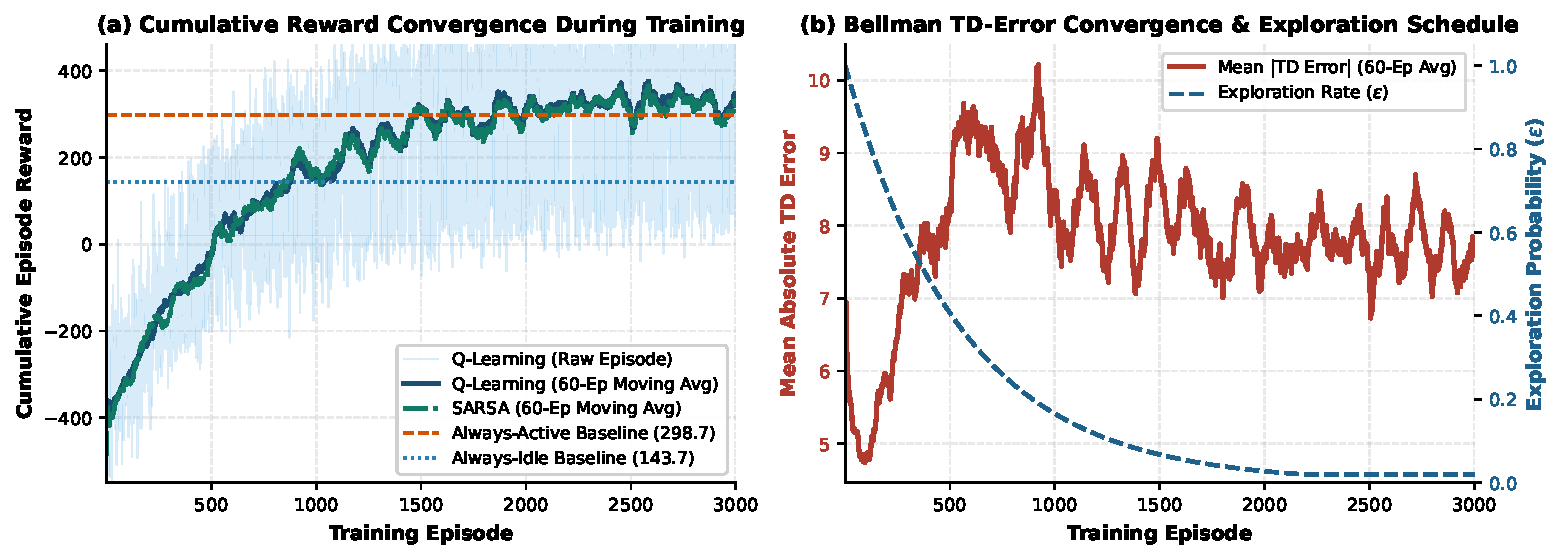
\includegraphics[width=0.98\columnwidth]{../figures/training_convergence.pdf}
    \caption{Training convergence over 3,000 episodes: (a) Cumulative episode reward for Q-Learning and SARSA surpassing static baselines; (b) Bellman TD-error stabilization alongside exponential $\epsilon$-decay.}
    \label{fig:training}
\end{figure}

\subsection{Environment Dynamics and Reward Function ($\mathcal{R}$)}
At step $t$, existing users depart via $n_{\text{dep},t} \sim \text{Binomial}(n_t, p_{\text{dep}}(h_t, d_t))$ and new requests arrive via a non-homogeneous Poisson process $n_{\text{arr},t} = \min(N - n_{\text{ret},t}, \text{Poisson}(\lambda(h_t, q_t, d_t)))$, where weekday $\lambda$ peaks at $5.2$ arrivals/step during afternoon labs ($14{:}00\text{--}18{:}00$) and drops to $0.04$ overnight. Step electrical energy (in kWh) combines active, standby, and transition overhead:
\begin{equation}
\begin{split}
    E_t &= \frac{N_{\text{srv},t} P_{\text{busy}} + (N - N_{\text{srv},t}) P_{\text{stby}}(a_t)}{1000}\Delta t + E_{\text{sw}}(m_t, a_t)
\end{split}
\end{equation}
where $E_{\text{sw}}(m_t, a_t) = 0.0035 (N - N_{\text{srv},t})(1 + 0.4(|a_t - m_t|-1))\mathbb{I}(a_t \neq m_t)$. Electricity cost is $C_t = c(h_t) E_t$ under a three-tier ToU tariff: $\$0.08/\text{kWh}$ off-peak ($21{:}00\text{--}06{:}00$), $\$0.12/\text{kWh}$ standard ($06{:}00\text{--}12{:}00$, $18{:}00\text{--}21{:}00$), and $\$0.18/\text{kWh}$ peak ($12{:}00\text{--}18{:}00$).

The multi-objective reward function $R_t$ is defined as:
\begin{equation}
\begin{split}
    R_t &= w_{\text{srv}} N_{\text{srv},t} - w_{\text{eng}} E_t - w_{\text{viol}} N_{\text{viol},t} \\
        &\quad - w_{\text{lat}} \left(\frac{L_t}{L_{\text{ref}}}\right) - w_{\text{sw}} \mathbb{I}(a_t \neq m_t)
\end{split}
\end{equation}
with weights $w_{\text{srv}}=1.25$ per served student-step, $w_{\text{eng}}=6.00/\text{kWh}$, $w_{\text{viol}}=6.50$ per violation, $w_{\text{lat}}=1.50$ ($L_{\text{ref}}=10.0\text{ s}$), and $w_{\text{sw}}=0.70$ per mode switch. When the lab is unoccupied with zero arrivals ($n_{\text{ret},t}=0, n_{\text{arr},t}=0$), user-experienced latency is $L_t = 0\text{ s}$.

\section{RL Algorithms \& Baseline Policies}
Because the state-action space has $|\mathcal{S}|\times|\mathcal{A}| = 720 \times 3 = 2,160$ entries, \textbf{Tabular Q-Learning} \cite{watkins1992q} is ideally suited: it avoids function-approximation divergence, guarantees convergence to $Q^*(s,a)$, and yields an inspectable policy table. At each transition $(s_t, a_t, R_t, s_{t+1})$, the off-policy TD(0) update is:
\begin{equation}
\begin{split}
    Q(s_t, a_t) &\leftarrow Q(s_t, a_t) + \alpha_k \Big[ R_t + \gamma (1 - d_{\text{done}}) \max_{a'\in\mathcal{A}} Q(s_{t+1}, a') \\
    &\quad - Q(s_t, a_t) \Big]
\end{split}
\end{equation}
We also train on-policy \textbf{Tabular SARSA}, replacing $\max_{a'} Q(s_{t+1},a')$ with $Q(s_{t+1}, a_{t+1})$ under the behavior policy. Both agents train for $K=3,000$ episodes ($288,000$ steps, training seed $42$) using $\epsilon$-greedy exploration with unvisited-action prioritization ($\epsilon_0=1.0 \to \epsilon_{\min}=0.02$, decay $\lambda_\epsilon=0.9982$) and learning rate decay ($\alpha_0=0.15 \to \alpha_{\min}=0.015$, $\lambda_\alpha=0.9992$). We compare against four baselines: (1) \textbf{\texttt{Always-Active}} ($a_t=2$), (2) \textbf{\texttt{Always-Idle}} ($a_t=1$), (3) \textbf{\texttt{Always-Sleep}} ($a_t=0$), and (4) \textbf{\texttt{Random}} ($a_t \sim \mathcal{U}\{0,1,2\}$).

\begin{figure}[t]
    \centering
    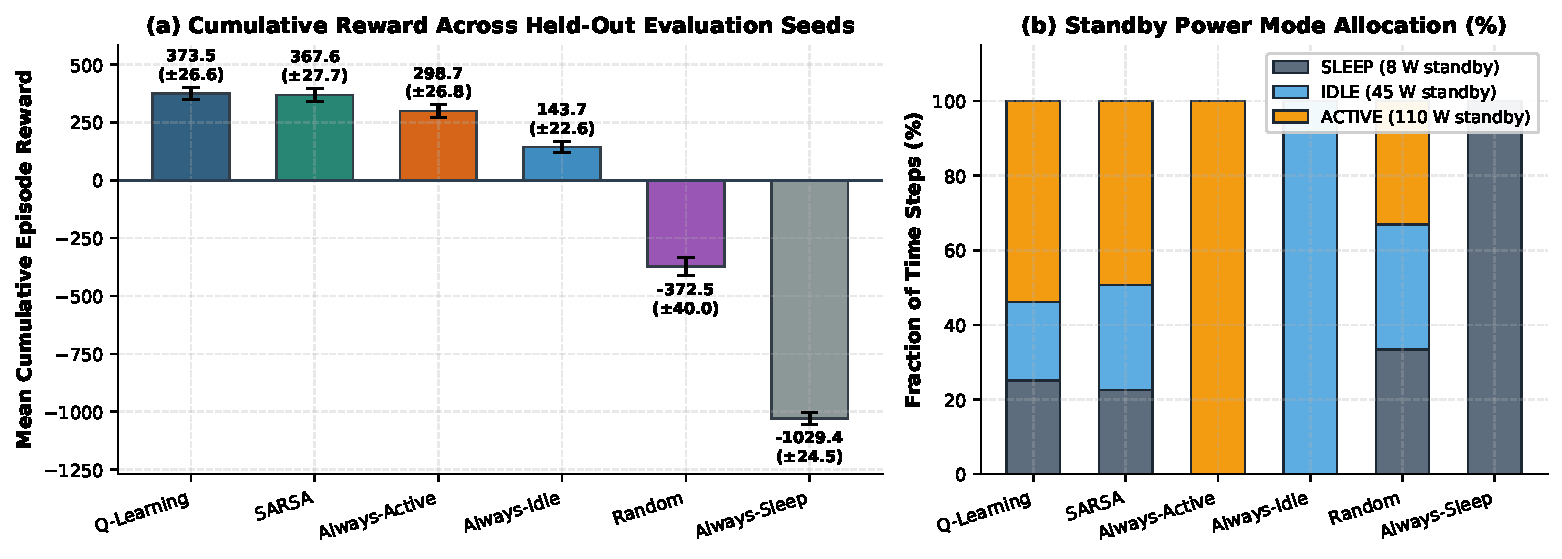
\includegraphics[width=0.98\columnwidth]{../figures/reward_comparison.pdf}
    \caption{Held-out evaluation across 20 seeds (100 episodes/policy): (a) Mean cumulative episode reward ($\pm 1\text{ SD}$); (b) Percentage of steps spent in \texttt{SLEEP}, \texttt{IDLE}, and \texttt{ACTIVE} modes.}
    \label{fig:reward}
\end{figure}

\begin{figure}[t]
    \centering
    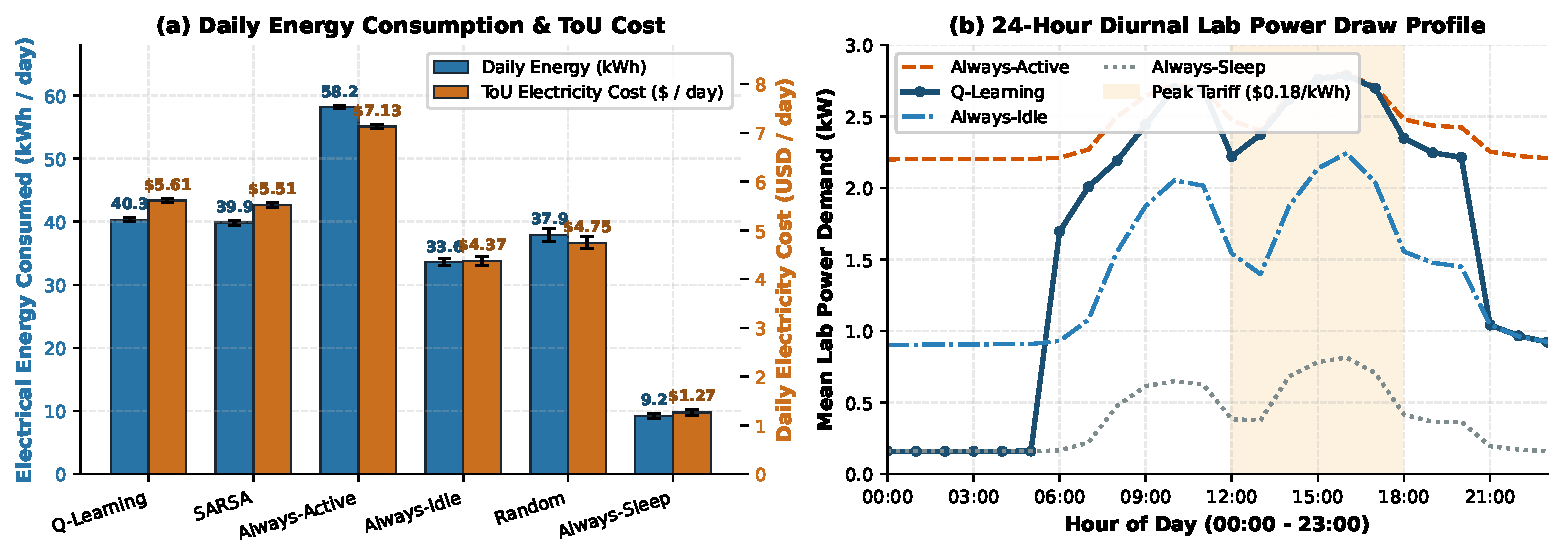
\includegraphics[width=0.98\columnwidth]{../figures/energy_and_cost.pdf}
    \caption{Energy and cost analysis: (a) Daily energy consumption (kWh) and ToU cost (\$); (b) 24-hour diurnal power profile showing Q-Learning sleeping overnight and scaling up for daytime labs.}
    \label{fig:energy}
\end{figure}

\begin{figure}[t]
    \centering
    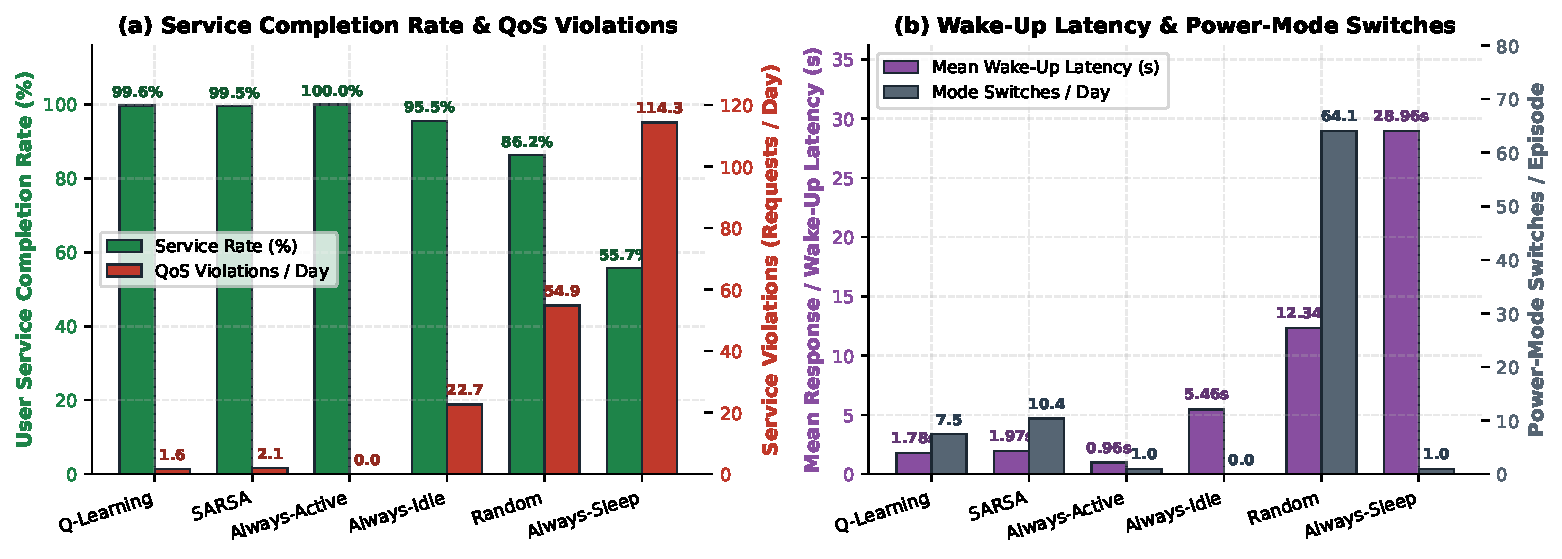
\includegraphics[width=0.98\columnwidth]{../figures/service_and_latency.pdf}
    \caption{Service quality metrics: (a) Student service completion rate (\%) and daily QoS violations; (b) Mean wake-up latency (s) and daily mode-switching frequency across policies.}
    \label{fig:service}
\end{figure}

\section{Experimental Evaluation \& Results}
To prevent training--evaluation leakage, evaluation is conducted on 20 strictly disjoint held-out random seeds (\texttt{1000..1019}), each running 5 episodes (4 weekdays + 1 weekend, totaling 100 episodes per policy) with greedy action selection ($\epsilon=0$).

\textbf{Training Convergence:} Fig.~\ref{fig:training}(a) shows that both Q-Learning and SARSA rapidly improve from $-362.9$ initial episode reward (under random exploration) to surpass \texttt{Always-Idle} ($143.7$) by episode $900$ and \texttt{Always-Active} ($298.7$) by episode $1,450$, converging smoothly as $\epsilon \to 0.02$ and mean TD error stabilizes (Fig.~\ref{fig:training}(b)). During training, $404/720$ physically reachable diurnal states are visited across $288,000$ updates.

\textbf{Quantitative Comparison:} Table~\ref{tab:results} and Figs.~\ref{fig:reward}--\ref{fig:service} summarize held-out performance across all metrics:
\begin{enumerate}[leftmargin=*,nosep,topsep=1pt]
    \item \textbf{Cumulative Reward:} \textbf{Q-Learning} achieves the highest reward of $\mathbf{373.52 \pm 26.64}$, outperforming \texttt{Always-Active} ($298.72$) by $\mathbf{+25.0\%}$ ($+74.80$ points) and \texttt{Always-Idle} ($143.74$) by $\mathbf{+159.9\%}$. On-policy \textbf{SARSA} achieves $367.60 \pm 27.70$, slightly more conservative due to accounting for exploratory risk during TD backups.
    \item \textbf{Energy \& Cost Reduction:} Compared to \texttt{Always-Active}, Q-Learning reduces daily energy consumption by $\mathbf{30.7\%}$ ($40.31$ vs.\ $58.17\text{ kWh/day}$, saving $17.86\text{ kWh/day}$ or $6,519\text{ kWh/year}$ per 20-PC lab) and lowers ToU electricity cost by $\mathbf{21.3\%}$ ($\$5.61$ vs.\ $\$7.13/\text{day}$). As shown in Fig.~\ref{fig:energy}(b), Q-Learning drops lab power to $0.16\text{ kW}$ (\texttt{SLEEP}) during $00{:}00\text{--}06{:}00$, tracks active lab demand during $08{:}00\text{--}20{:}00$, and ramps down to $0.95\text{ kW}$ (\texttt{IDLE}) after $21{:}00$.
    \item \textbf{QoS, Violations \& Latency:} Q-Learning serves $525.4$ requests/day ($\mathbf{99.6\%}$ service rate) with only $1.61$ violations/day and $1.78\text{ s}$ mean latency---eliminating $92.9\%$ of the violations incurred by \texttt{Always-Idle} ($22.70$/day, $5.46\text{ s}$) and $98.6\%$ of those under \texttt{Always-Sleep} ($114.33$/day, $28.96\text{ s}$). Moreover, Q-Learning executes only $7.50$ mode switches/day (vs.\ $64.07$ for \texttt{Random}).
\end{enumerate}

\section{Discussion, Limitations \& Conclusion}
Fig.~\ref{fig:heatmap} and Fig.~\ref{fig:reward}(b) reveal the learned multi-regime strategy $\pi^*(s)$: Q-Learning selects \texttt{SLEEP} ($25.2\%$ of steps) during empty overnight periods ($00{:}00\text{--}06{:}00$), \texttt{IDLE} ($20.8\%$ of steps) during low-load midday/evening blocks and weekend study hours, and proactively switches to \texttt{ACTIVE} ($54.0\%$ of steps) during weekday lab periods to absorb bursty student arrivals without wake-up timeouts.

\begin{figure}[h!]
    \centering
    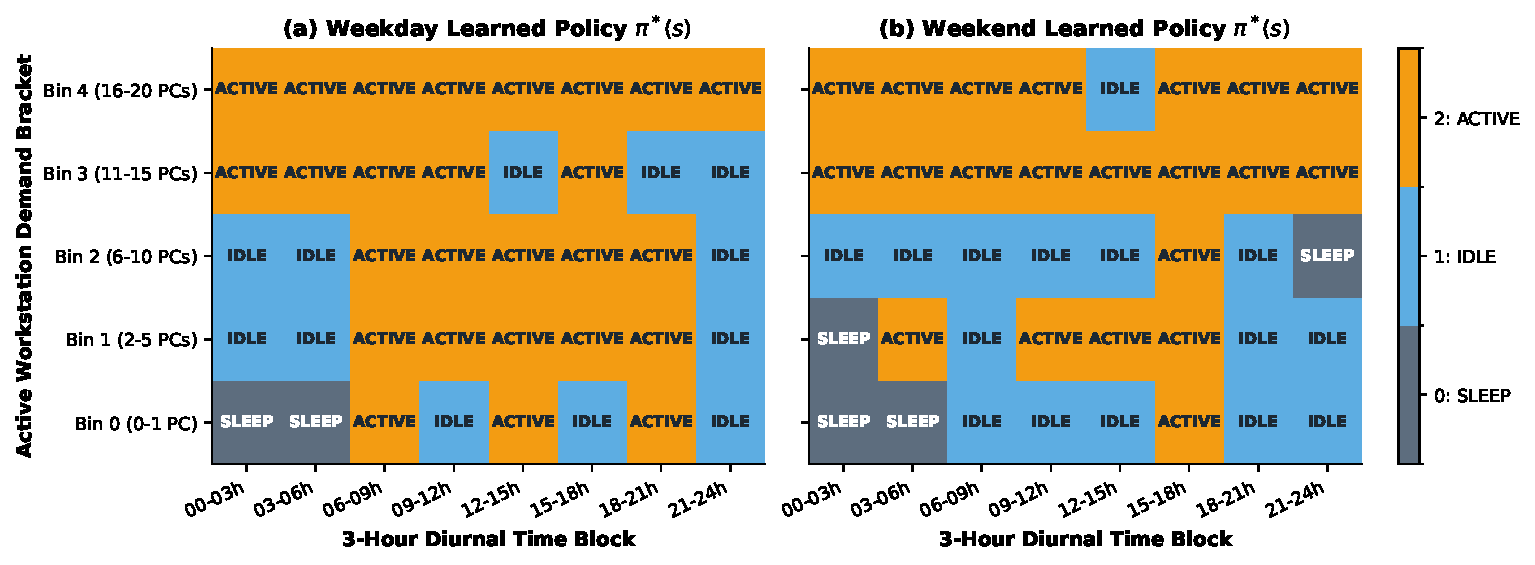
\includegraphics[width=0.98\columnwidth]{../figures/learned_policy_heatmap.pdf}
    \caption{Learned greedy Q-Learning policy $\pi^*(s)$ across diurnal blocks and occupancy brackets for (a) Weekdays and (b) Weekends.}
    \label{fig:heatmap}
\end{figure}

\textbf{Limitations \& Future Work:} Our current environment applies a unified standby mode across all unoccupied PCs and assumes homogeneous workstation hardware. Extending the action space to fine-grained cluster sizing (maintaining a dynamic warm-idle buffer of $k \in \{0,\dots,N\}$ PCs) using Deep Q-Networks (DQN) \cite{mnih2015human} conditioned on academic calendar deadlines is a promising direction.

\newpage
\onecolumn
\begin{thebibliography}{9}
\small

\bibitem{sutton2018reinforcement}
R.~S. Sutton and A.~G. Barto, \emph{Reinforcement Learning: An Introduction}, 2nd~ed.\hskip 1em plus 0.5em minus 0.4em\relax Cambridge, MA, USA: MIT Press, 2018.

\bibitem{watkins1992q}
C.~J. C.~H. Watkins and P.~Dayan, ``Q-learning,'' \emph{Machine Learning}, vol.~8, no. 3--4, pp. 279--292, May 1992.

\bibitem{benini1999policy}
L.~Benini, A.~Bogliolo, G.~A. Paleologo, and G.~De~Micheli, ``Policy optimization for dynamic power management,'' \emph{IEEE Transactions on Computer-Aided Design of Integrated Circuits and Systems}, vol.~18, no.~6, pp. 813--833, Jun. 1999.

\bibitem{qiu2001dynamic}
Q.~Qiu, Q.~Wu, and M.~Pedram, ``Stochastic modeling of a power-managed system---Construction and optimization,'' \emph{IEEE Transactions on Computer-Aided Design of Integrated Circuits and Systems}, vol.~20, no.~10, pp. 1200--1217, Oct. 2001.

\bibitem{tesauro2007reinforcement}
G.~Tesauro, N.~K. Jong, R.~Das, and M.~N. Bennani, ``On the use of hybrid reinforcement learning for autonomic resource allocation,'' \emph{Cluster Computing}, vol.~10, no.~3, pp. 287--299, Sep. 2007.

\bibitem{mnih2015human}
V.~Mnih \emph{et~al.}, ``Human-level control through deep reinforcement learning,'' \emph{Nature}, vol. 518, no. 7540, pp. 529--533, Feb. 2015.

\end{thebibliography}

\end{document}
